\section{Activation of RTK}

The \SBGNERLone language is designed under the ``open world'' assumption. Under this assumption, all entities, state variables and interactions are assumed to be independent, unless explicitly specified with influence arc. This approach helps to avoid a combinatorial explosion of the states represented in the map and makes drawing diagrams much easier compared to \SBGNPDLone, but it makes reading and analysis of the diagram more difficult.  

To illustrate creation and analysis of \SBGNERLone diagram we will create the diagram of receptor tyrosine kinase (RTK) activation pathway in a step by step manner. Wikipedia (\url{https://en.wikipedia.org/wiki/Receptor_tyrosine_kinase}) describes the process of RTK activation as follows:
\begin{quote}
``When a growth factor binds to the extracellular domain of an RTK, its dimerization is triggered with other adjacent RTKs. Dimerization leads to a rapid activation of the protein's cytoplasmic kinase domains, the first substrate for these domains being the receptor itself. The activated receptor as a result then becomes autophosphorylated on multiple specific intracellular tyrosine residues.''
\end{quote}

Drawing \SBGNERLone diagrams is simple, we will follow the textual description of the pathway and add required elements. Let's start with identification of key players of the pathway. From the text, we can determine that the two main entities are ``RTK'' and ``growth factor''. We will draw them as ``receptor'' and ``ligand''  entities (\sect{entity}), respectively. We also notice that RTK has two domains: the ``extracellular domain'' (``receptor'') and the ``kinase domain'', they will also be shown in \fig{rtk-entities}. The pathway description also mentions ``multiple specific intracellular tyrosine residues'', so we have added two state variables (\sect{stateVariable}) ``Y1'' and ``Y2''' to the receptor entity to be able to show events related to modification of the tyrosine residues.  

\begin{figure}[H]
  \centering
  \vspace*{-0.75em}
  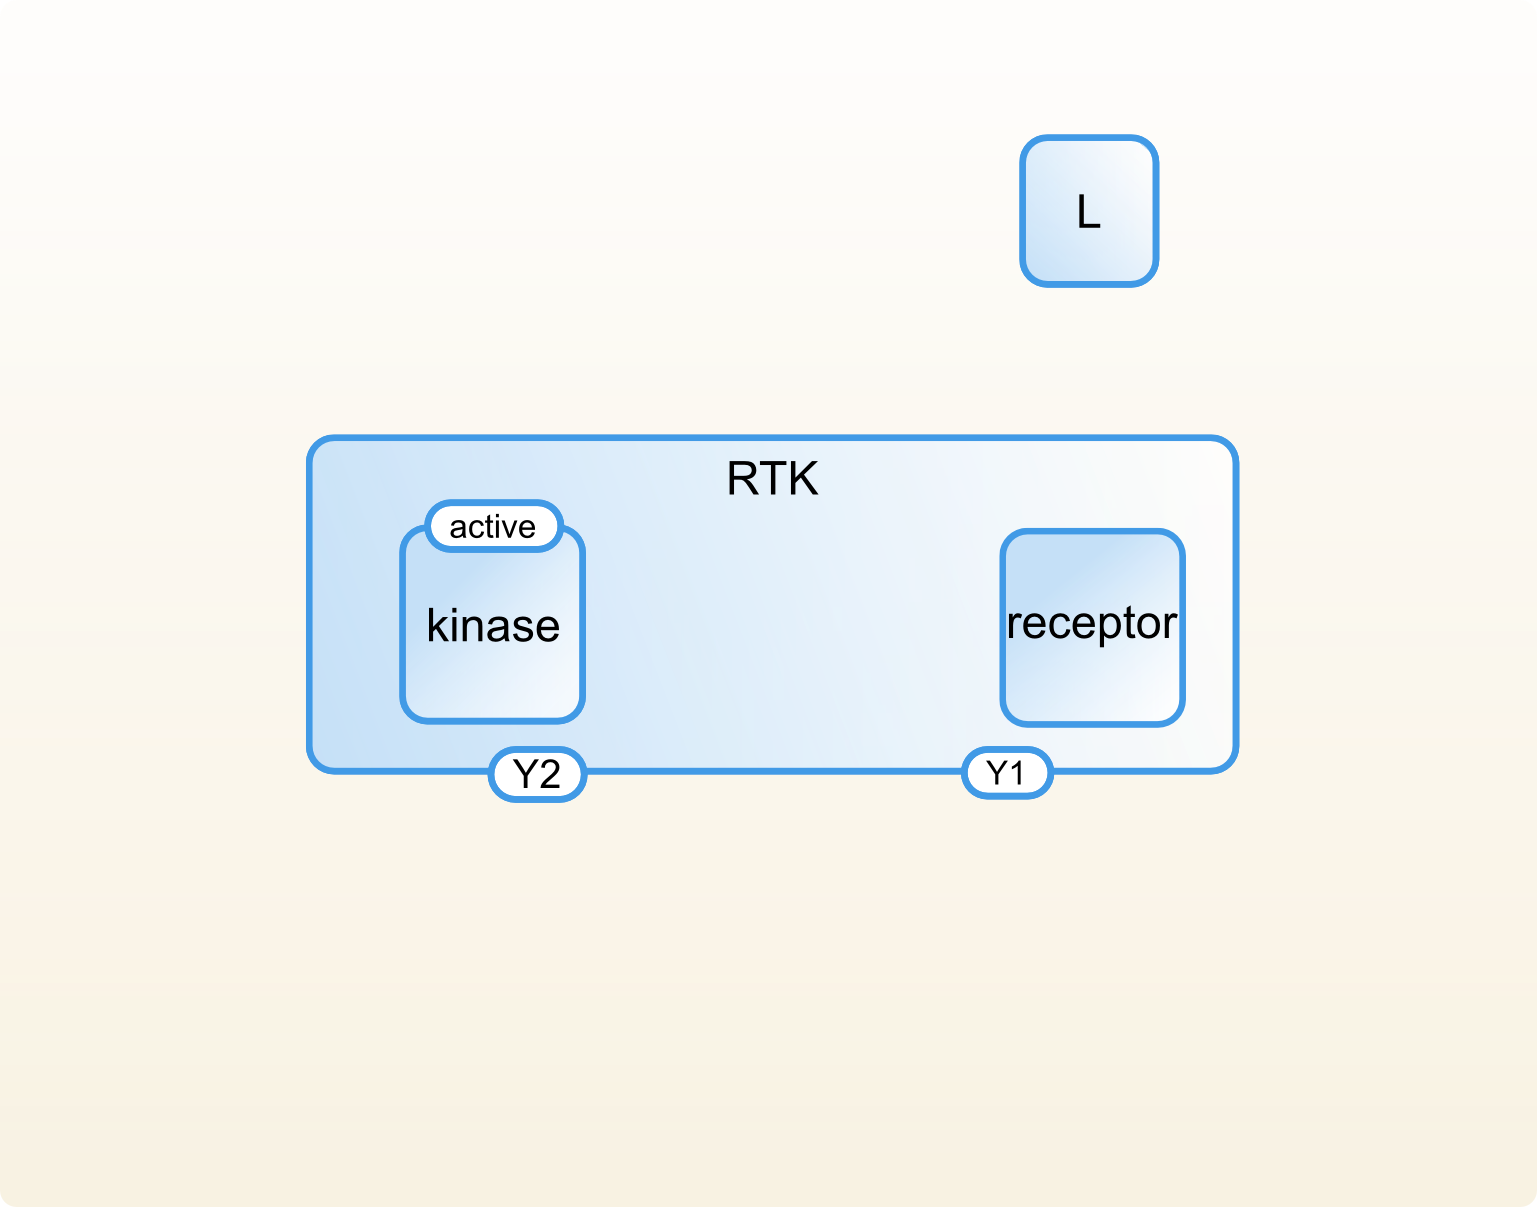
\includegraphics[scale=0.75]{examples/rtk-entities.png}
   \caption{Receptor tyrosine kinase activation: definition of entities.}
  \label{fig:rtk-entities}
\end{figure}

Through this entity creation process, we have populated our system with instances of two kinds: a ``receptor'' and a ``ligand''. We also show the internal structure of the receptor by depicting its two domains as nested entities (\sect{domain}). The receptor and its ``kinase'' domain have ``state variables'' (\sect{stateVariable}) that define the basis for the entity state space.

We will now describe the entity state space for each entity that we are interested in. The two assignment arcs (\sect{assignment}) pointing to the ``Y1'' and ``Y2'' receptor state variables on \fig{rtk-states} demonstrate that we are going to analyse phosphorylation of tyrosine residues. From the statement: ``Dimerization leads to a rapid activation of the protein's cytoplasmic kinase domains'', we need to take into account that the ``active'' state variable of ``kinase'' domain could become ``true'' after some perturbations in the system. Therefore, we have added an appropriate variable value (\sect{variableValue}) node and an assignment arc.

Given that the \SBGNERLone follows the ``open world'' assumption, diagram authors are not obliged to describe the entire system, and we can focus on the most important parts of the system. For this reason, we include only the ``P'' state value for the residues. For a more accurate description of the system, we need to include a default value, such as the ``unphosphorylated'' state (see \sect{assignment} to check how to do it properly), but in our case it is not important so we will rely on the ``open world'' assumption and omit this detail.  \SBGNERLone assumes that all interactions are internally reversible, so if we only describe the switch from default to phosphorylated state explicitly, that description implies that there is a mechanism to put ``Y1'' and ``Y2'' variables back to their default state. For the same reason,  we have not added ``false'' value to the ``active'' state of the kinase domain.
 
\begin{figure}[H]
  \centering
  \vspace*{-0.75em}
  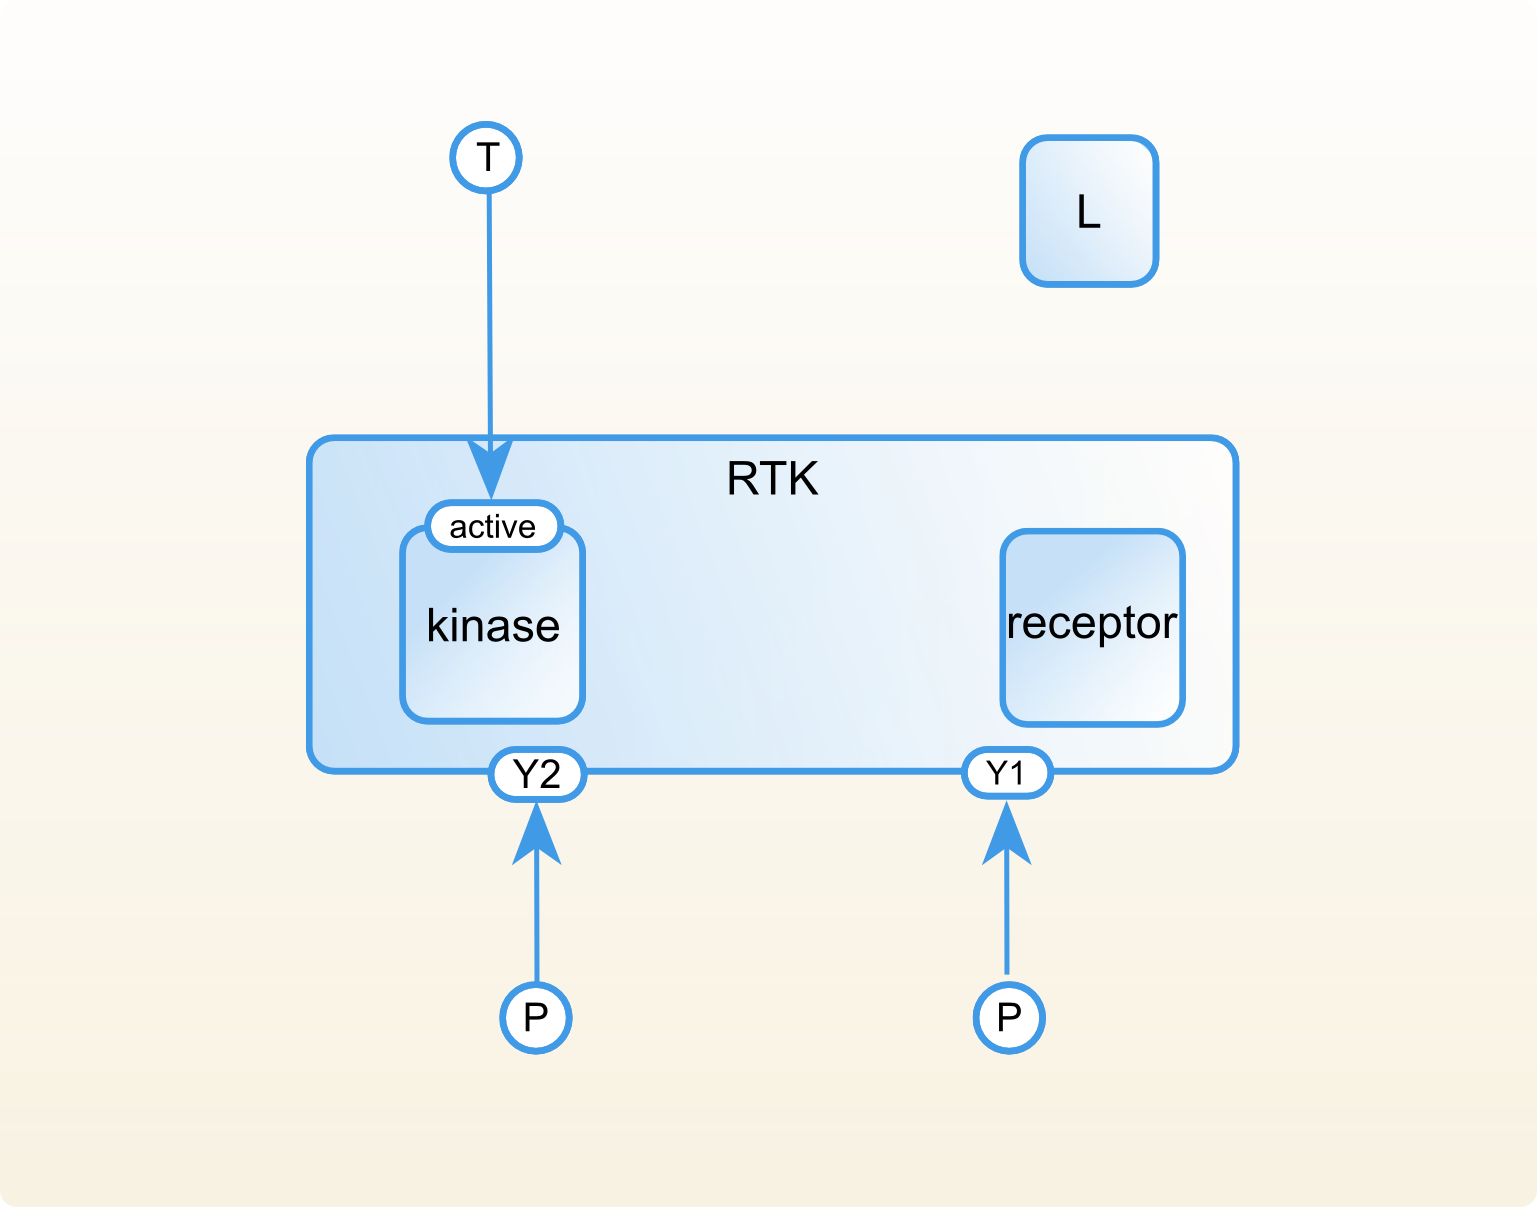
\includegraphics[scale=0.75]{examples/rtk-states.png}
   \caption{Receptor tyrosine kinase activation: state variable assignment.}
  \label{fig:rtk-states}
\end{figure}

We have now prepared all elements that are taking part in the process, and we are ready to draw the pathway itself. The first sentence of the pathway description states ``When a growth factor \textbf{binds} to the extracellular domain of an RTK'', so the first event we are going to draw is a receptor ligand binding (\fig{rtk-binding}). We will use an interaction arc (\sect{interaction}) to show that the ligand can bind the receptor.

\begin{figure}[H]
  \centering
  \vspace*{-0.75em}
  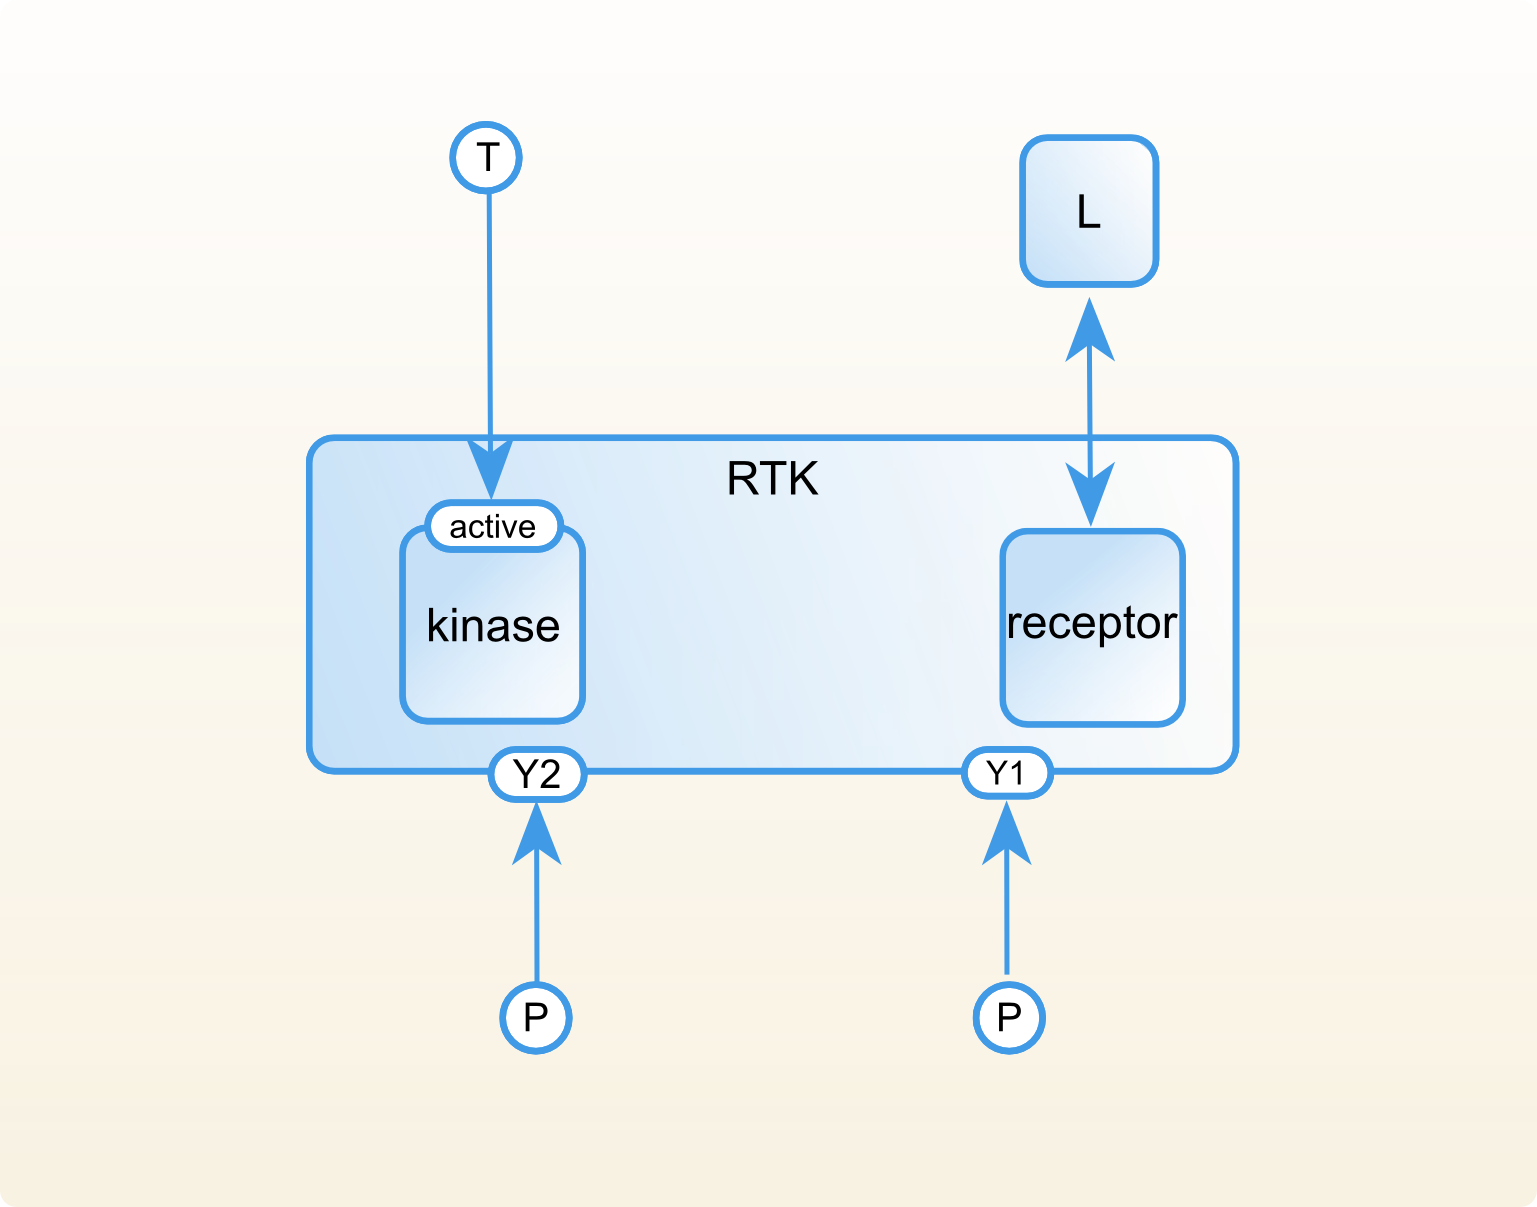
\includegraphics[scale=0.75]{examples/rtk-binding.png}
   \caption{Receptor tyrosine kinase activation: receptor-ligand binding.}
  \label{fig:rtk-binding}
\end{figure}

The binding happens between the ligand entity and the receptor domain of the RTK entity. The interaction event is reversible in a same way as assignment. That means that even if two instances of ligand and receptor are bound at some time that bond will not last forever, it will dissociate with some probability.

The next statement in the description is ``When a growth factor binds to the extracellular domain of an RTK, its \textbf{dimerisation} is triggered with other adjacent RTKs''. The dimerisation event is added in \fig{rtk-dimerisation}. The interaction arc connects the entity with itself, so we need to distinguish two possibilities: 1) the receptor molecule binds another molecule of the same kind (what we need according to the pathway description) or 2) that RTK undergoes an intramolecular interaction. In the first case, we add a \glyph{unit of information} ``trans'' to the arc to emphasise that the interaction is intermolecular. The second case would require \glyph{unit of information} ``cis'' (see \sect{unitInformation}, \sect{miscellaneous-cv} and \sect{cis-trans-semantics}). Definition of ``cis'' or ``trans'' interaction is meaningful only for events involving instances of the same entity occurring directly or via chain of events. If you do not specify cis/trans type of interaction, this information will be undefined, because of the ``open world'' nature of \SBGNERLone. This is correct and sometimes unavoidable, but the diagram is more understandable when the appropriate \glyph{unit of information} is added to the interaction arc in accordance with biological knowledge.

\begin{figure}[H]
  \centering
  \vspace*{-0.75em}
  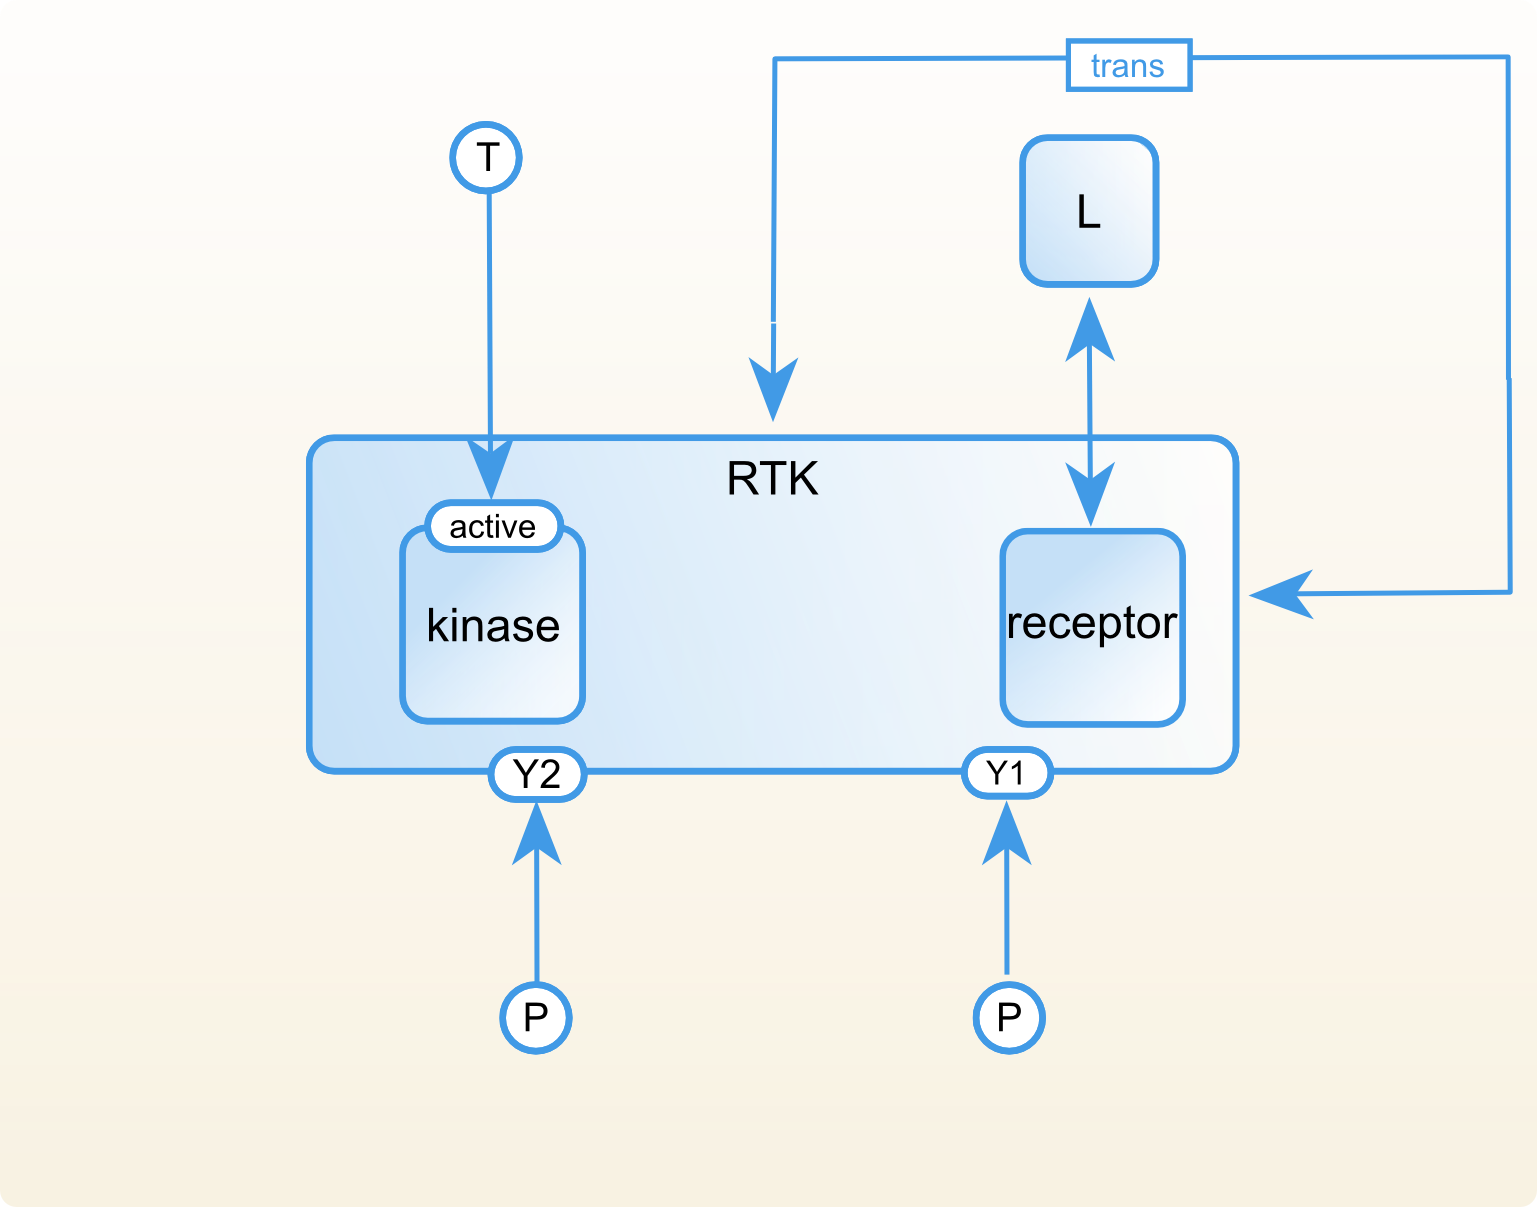
\includegraphics[scale=0.75]{examples/rtk-dimerisation.png}
   \caption{Receptor tyrosine kinase activation: receptor dimer formation.}
  \label{fig:rtk-dimerisation}
\end{figure}

Now, we have to emphasise that the dimerisation depends upon the ligand-receptor binding. There are two key elements of \SBGNERLone we will use in this step (see \fig{rtk-dimer-control}): outcome (\sect{outcome}) and influence arc (\sect{influences}). In our case the result of interaction is a complex containing instances of receptor and ligand, but this is not limited to the binary complex, as we will see soon. To show the results of an interaction on the diagram an outcome node is placed on the on the interaction arc, as a black dot. This outcome dot is the origin of our influence arc (\sect{influences}). Influence arcs are designed to depict the way one part of the system controls the behaviour of the other. The word ``triggered'' in a pathway description implies that the interaction between receptor and ligand is necessary for the dimerisation process, so we have used necessary stimulation (\sect{necessaryStimulation}), which indicates that without the stimulator entity the target interaction cannot take place. Furthermore, we have placed ``cis'' \glyph{unit of information} on the influence arc to emphasise that the control happens within the same molecular complex. That means that the receptor-ligand complex is a member of the formed dimer.
 
\begin{figure}[H]
  \centering
  \vspace*{-0.75em}
  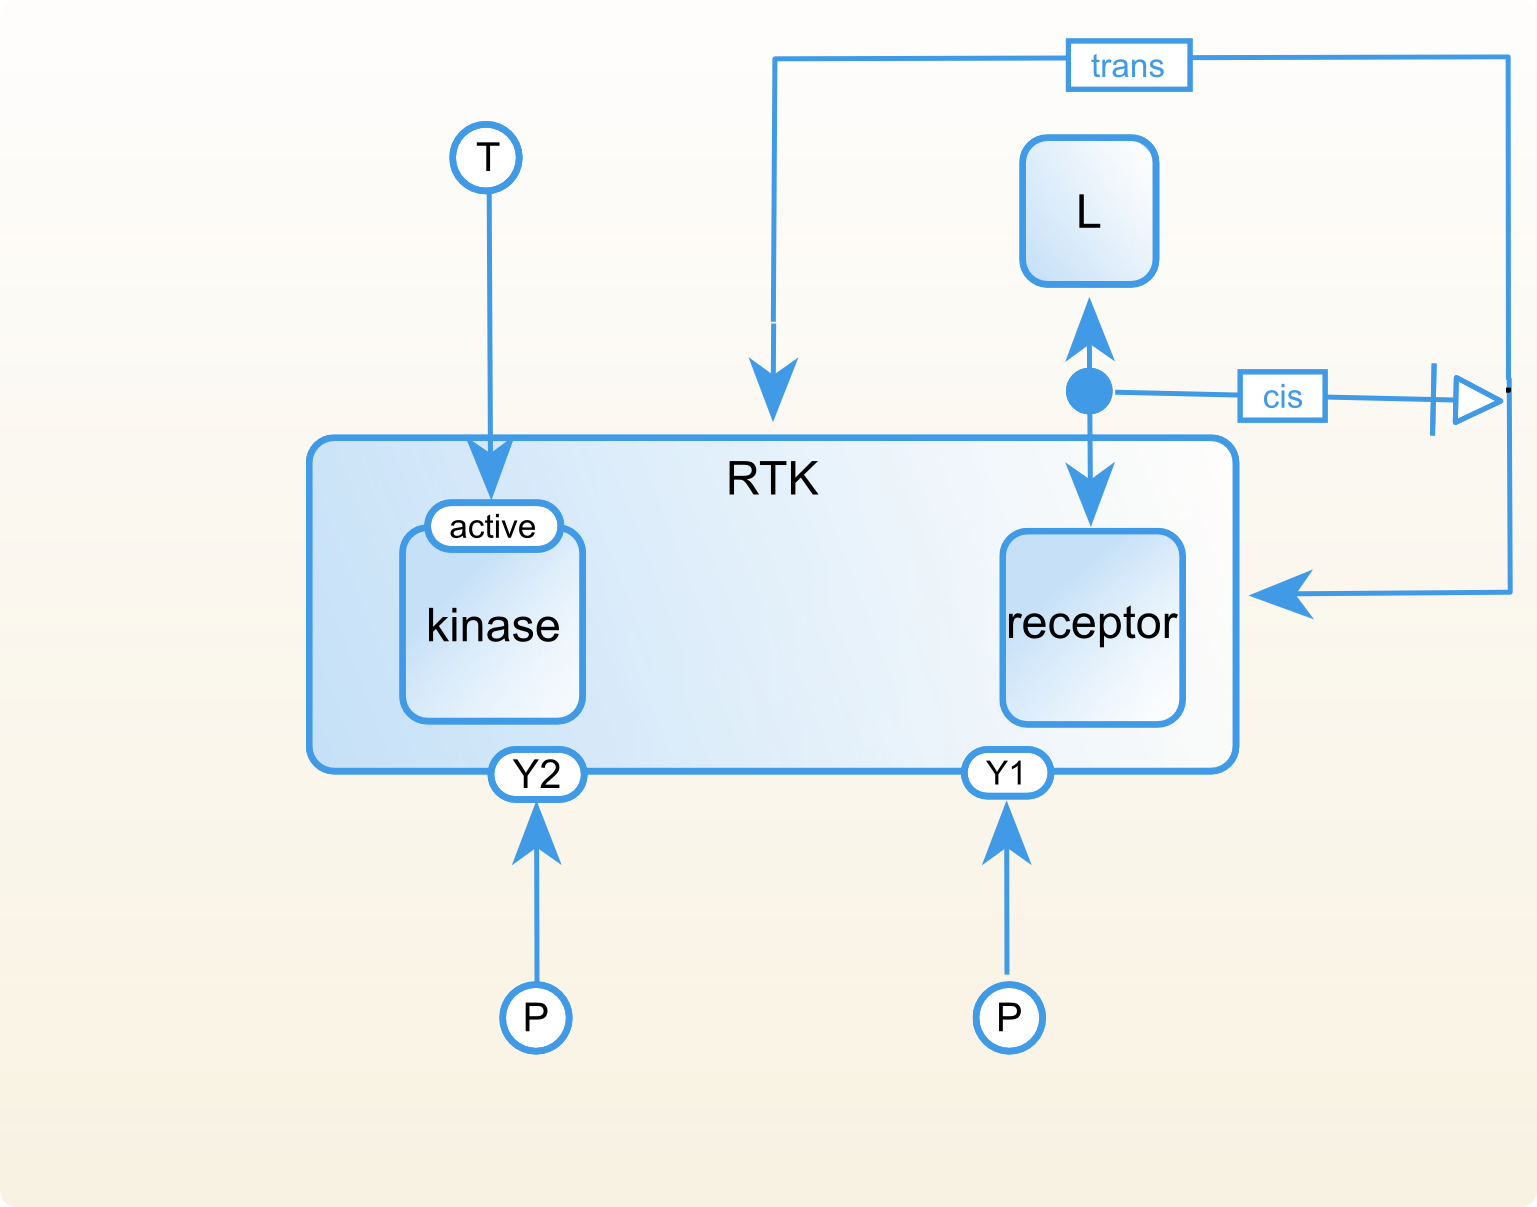
\includegraphics[scale=0.75]{examples/rtk-dimer-control.png}
   \caption{Receptor tyrosine kinase activation: control of the dimer formation.}
  \label{fig:rtk-dimer-control}
\end{figure}

The next sentence in the description states: ``Dimerization leads to a rapid activation of the protein's cytoplasmic kinase domains,''. In \fig{rtk-kinase-activation}, we will add another influence arc, stimulation (\sect{stimulation}) that means the kinase domain may be active to some extent even in monomeric form of a receptor. On the dimerisation interaction, we again have an outcome dot to represent the dimer, as the source of the influence arc, but in this case the outcome represents any kind of complex where two receptor molecules bound together.

\begin{figure}[H]
  \centering
  \vspace*{-0.75em}
  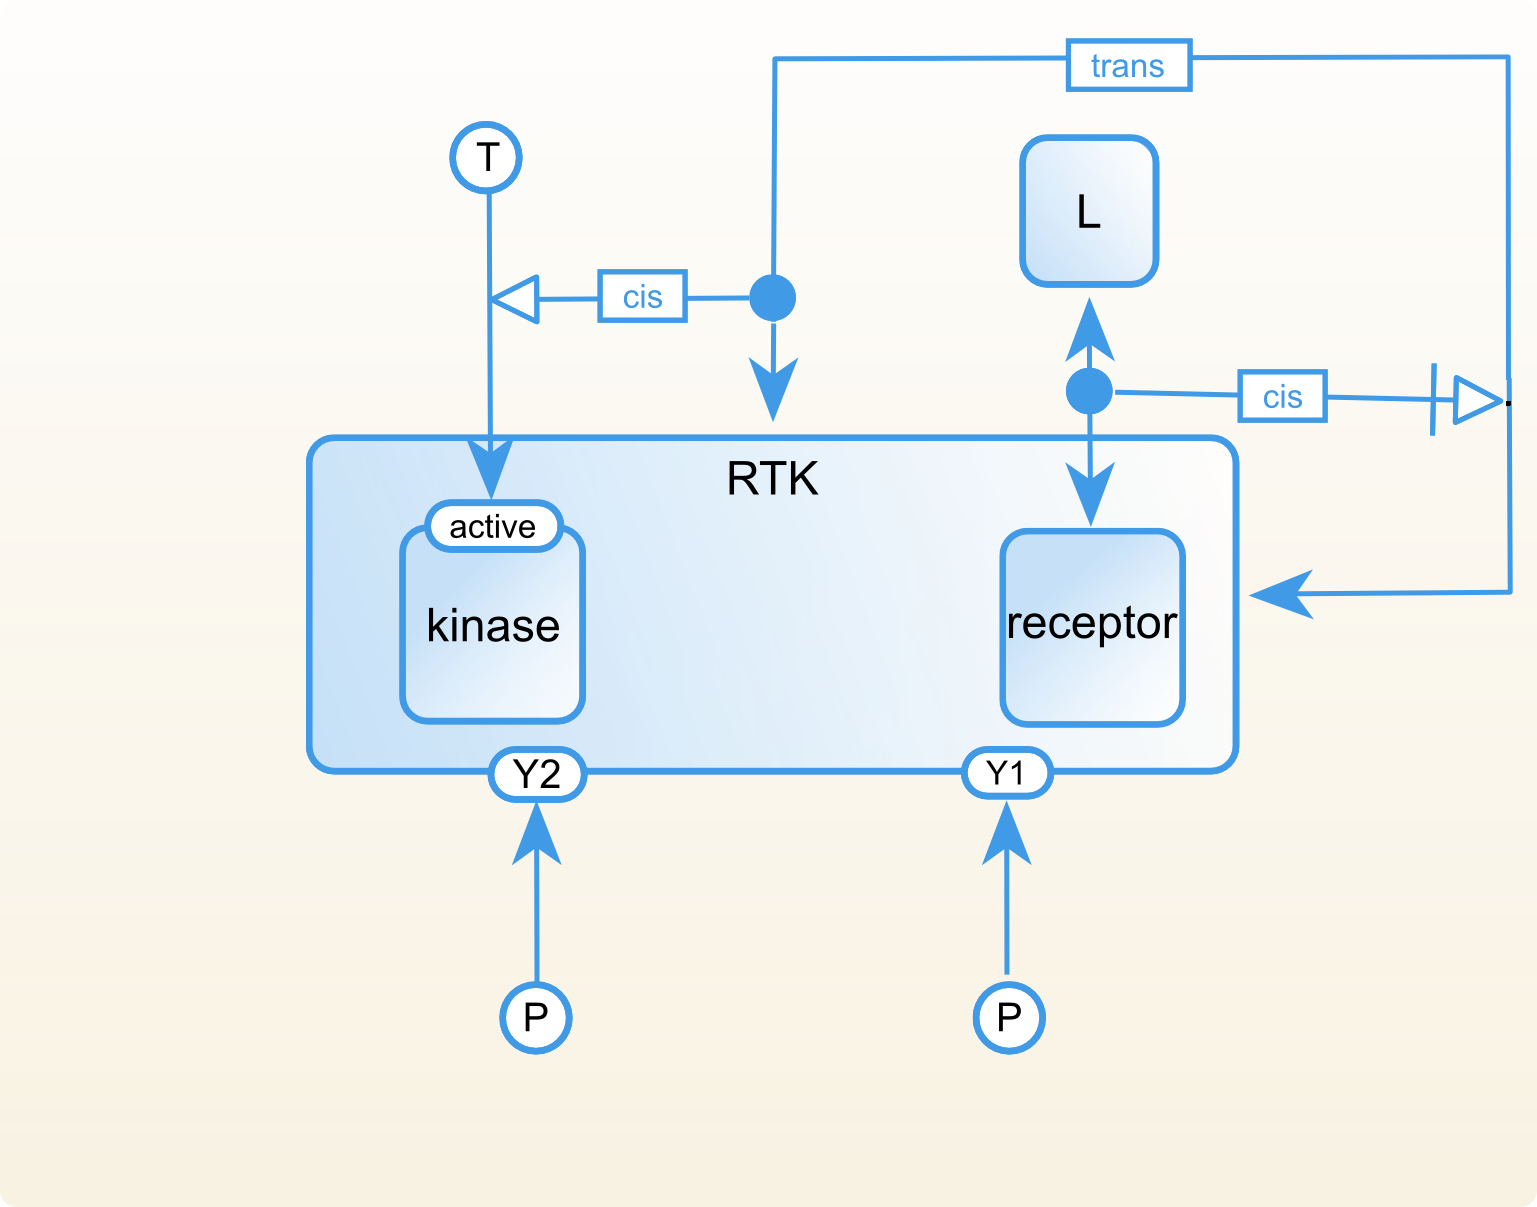
\includegraphics[scale=0.75]{examples/rtk-kinase-activation.png}
   \caption{Receptor tyrosine kinase activation: activation of the kinase domain of the receptor.}
  \label{fig:rtk-kinase-activation}
\end{figure}

The last part of our pathway is the ``autophosphorylation of multiple specific intracellular tyrosine residues'' by activated kinase domain. The complete pathway is shown in \fig{rtk-full}. All interactions and influences in \SBGNERLone are independent, so each stimulation arc representing autophosphorylation of the tyrosine residue has its own outcome, and these outcomes represent independent sets of instances where kinase is active.

\begin{figure}[H]
  \centering
  \vspace*{-0.75em}
  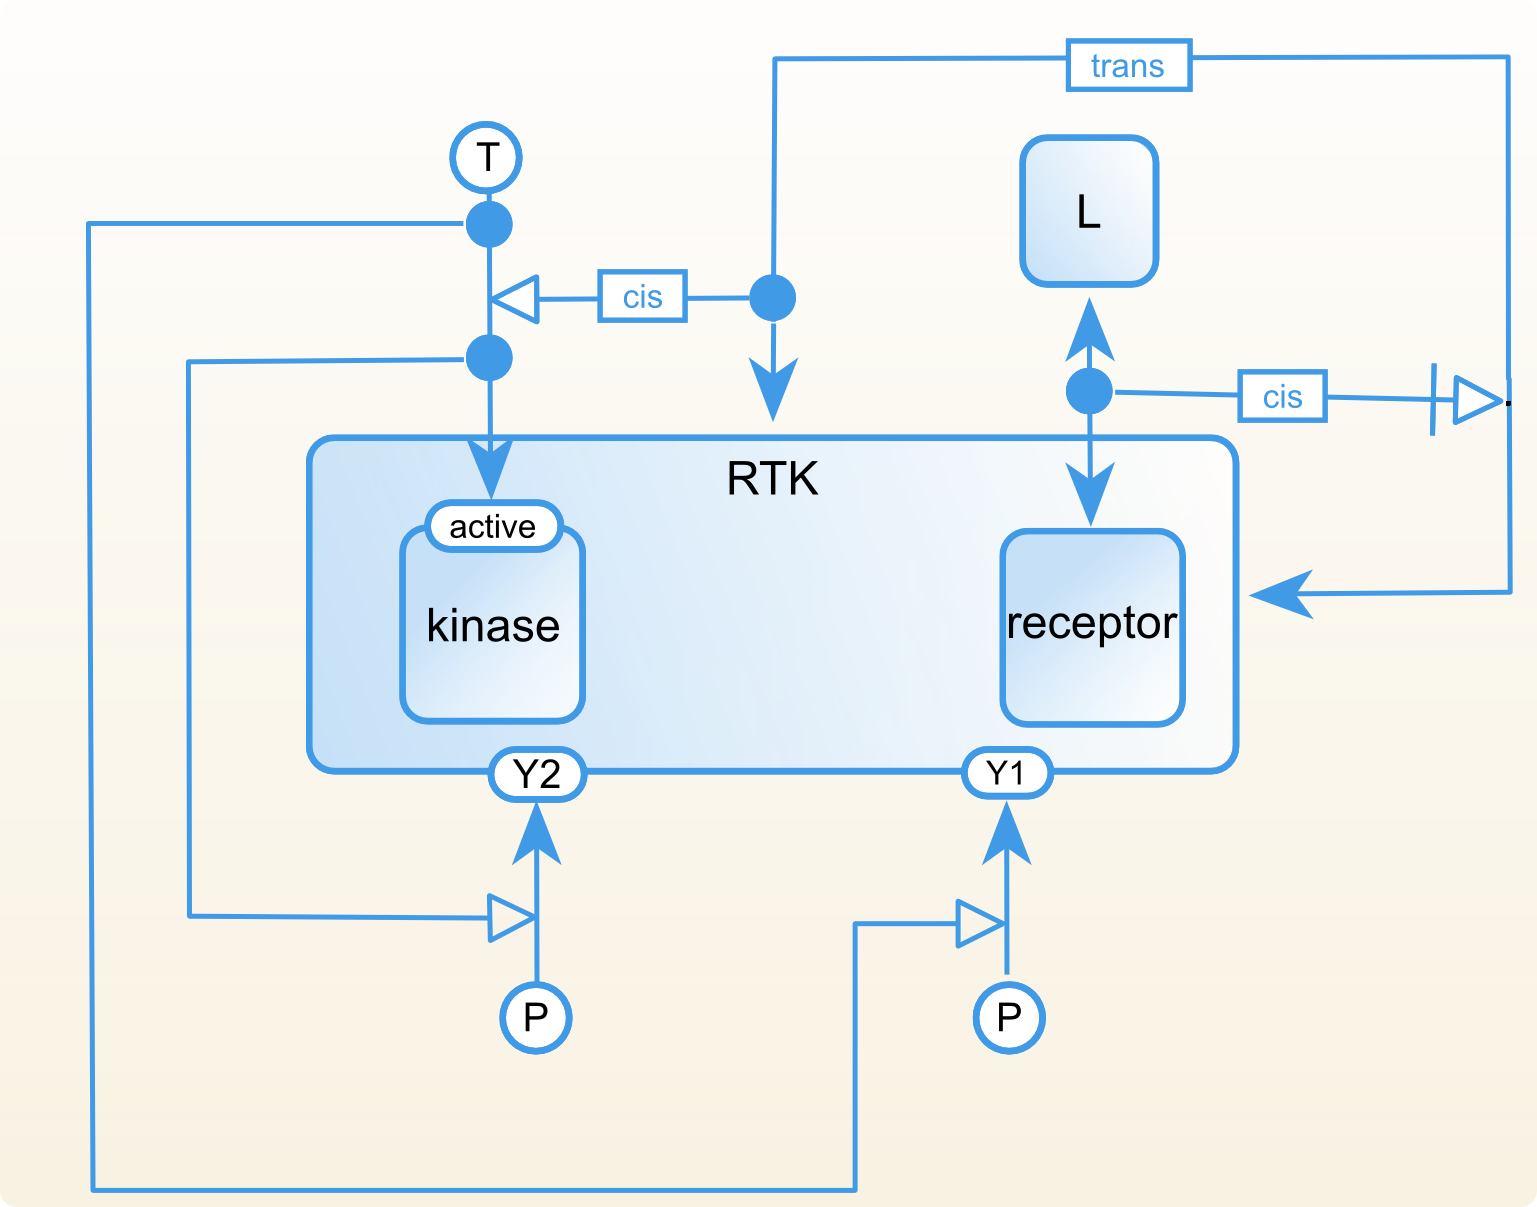
\includegraphics[scale=0.75]{examples/rtk.png}
   \caption{The complete diagram of receptor tyrosine kinase activation.}
  \label{fig:rtk-full}
\end{figure}

Now that our diagram is ready let's analyse it to get a better understanding of rules of the language and meaning of the diagram elements. The diagram consists of two types of entities, three types of outcomes, two interaction arcs, three assignment arcs, and four influence arcs. If we take into account independence and reversibility of all interactions we can count the total number of complexes that could be created in the system. It will be 153 complex types in total: 8 monomeric receptors, 8 monomeric receptor-ligand complexes, 36 receptor dimers, 64 receptor dimers with one ligand, 36 receptor dimers with two ligands and free ligand. Those numbers come from simple combinatorics, taking into account the number of state variables and assuming that each of them can have two values: ``undefined'' or specified by assignment arc. \fig{rtk-complexes} shows three of the 144 complexes compatible with the defined outcome.

\begin{figure}[H]
  \centering
  \vspace*{-0.75em}
  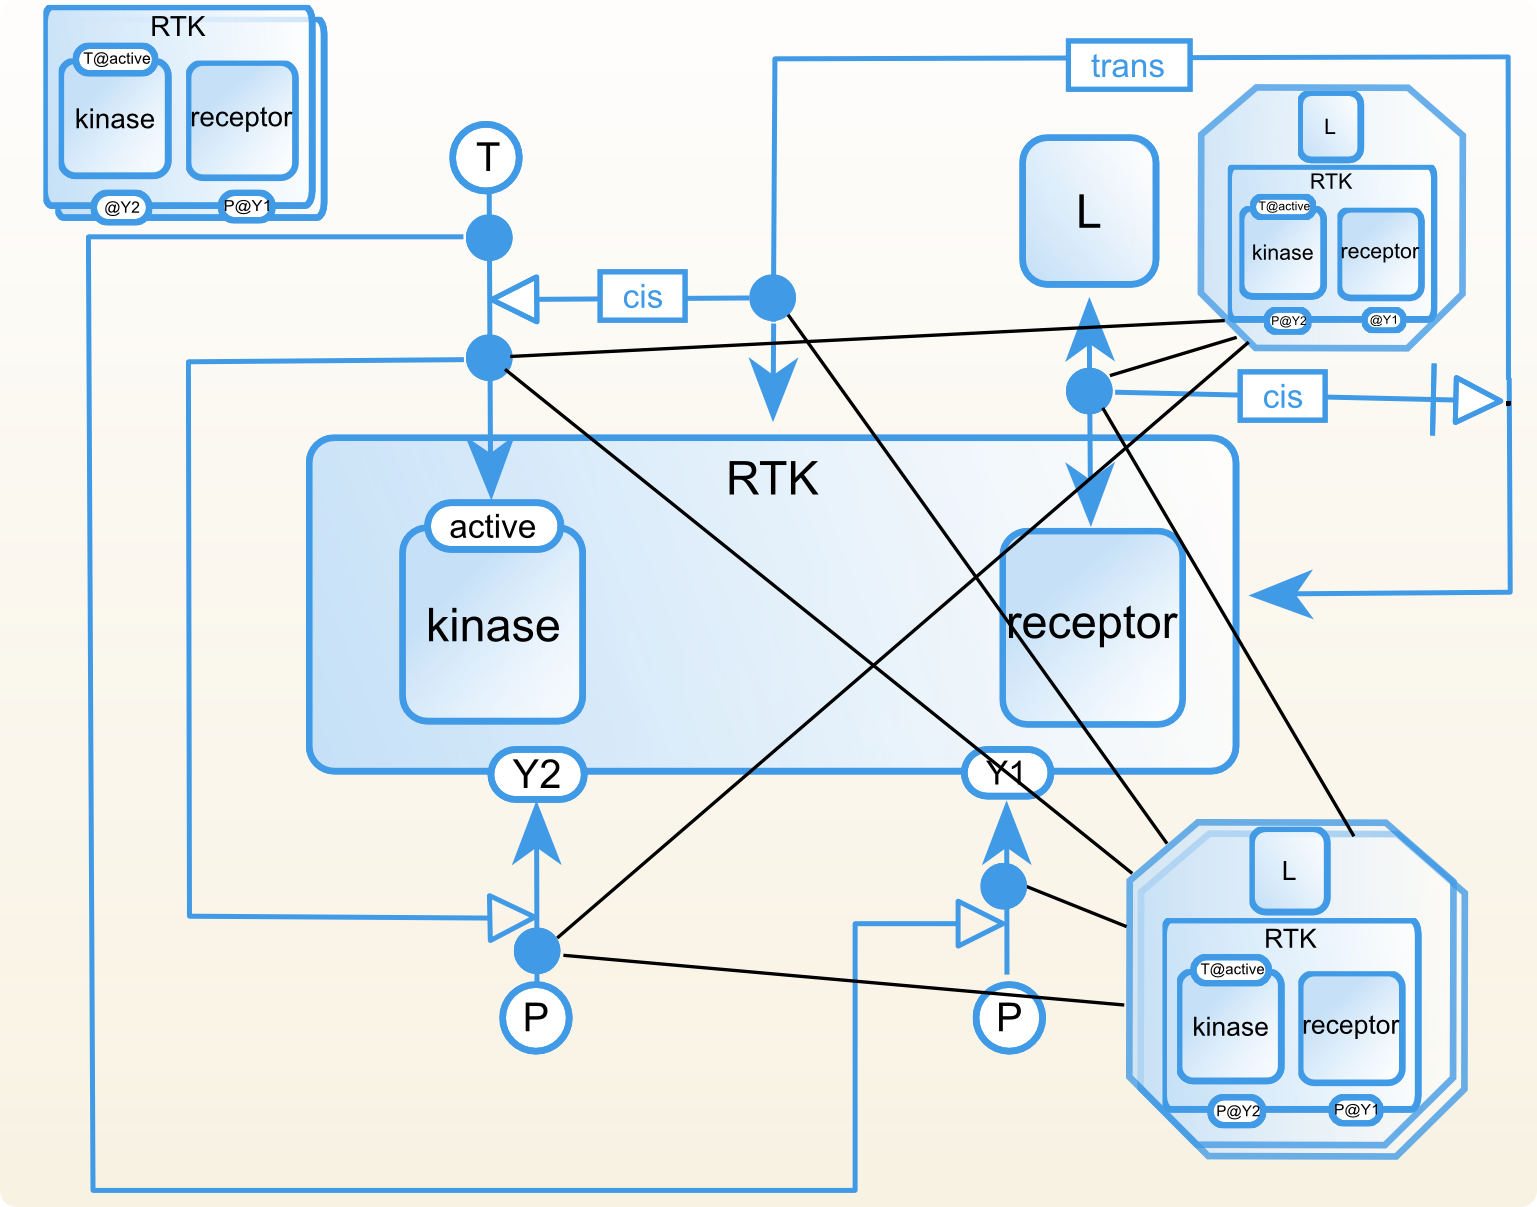
\includegraphics[scale=0.75]{examples/rtk-complex.png}
   \caption{Receptor tyrosine kinase activation: examples of active kinase complexes are shown. Black lines connect two complexes with outcomes, which definition is compatible with the complex status.}
  \label{fig:rtk-complexes}
\end{figure}

The large number possible complexes is defined by the influence arcs, which dictate the number of available states. For example, blocking any single phosphorylation site reduces the number of reachable complexes to 45, and blocking the kinase activation reduces the total set of possible complexes types to just 6. This can easily be seen from the diagram. In the first case, we switch off one receptor state variable, and in the second case, we effectively block all three; blocking activation assignment we render all its outcomes to false state. This means that activation will never happen and that the tyrosine residues will never be phosporylated. In the next section, we will present more complex examples. 
